\documentclass[14pt, a4paper]{report}
\usepackage{mathtext}
\usepackage[T2A]{fontenc}
\usepackage[utf8]{inputenc}
\usepackage[russian]{babel}
\usepackage{multirow}
\usepackage{slashbox}
\usepackage{makecell}
\usepackage{graphicx}
\usepackage{physics}
\usepackage{amstext}
\usepackage{caption}
\usepackage{subcaption}
\usepackage{cmap}
\usepackage{float}
\usepackage{siunitx}

\renewcommand{\thesection}{\arabic{section}.}
\renewcommand{\thesubsection}{\arabic{section}.\arabic{subsection}.}

\title{\textbf{Отчет о выполнении лабораторной работы 4.6.2 "Туннелирование миллиметровых радиоволн"}}
\author{Алпатова Александра, Калашников Михаил, Б03-205}
\date{}

\begin{document}
\maketitle

\textbf{Цель работы:}
экспериментальное исследование эффекта проникновения электромагнитных волн -- туннелирования -- через воздушный зазор между диэлектрическими призмами при полном внутреннем отражении на границе диэлектрик-воздух, а также моделирование интерферометра Майкельсона с использованием этого эффекта и измерение длины волны излучения и показателя преломления фторопласта для радиоволн миллиметрового диапазона.
\newline

\textbf{В работе используются:}
\begin{itemize}
\item генератор СВЧ-колебаний с рупорной антенной;
\item приемная рупорная антенна и волновод;
\item детектор;
\item микроамперметр;
\item Металлические зеркала;
\item две призмы и плоскопараллельная пластина из фторопласта;
\item микрометрические винты.
\end{itemize}

\section{Экспериментальная установка}

Туннелирование миллиметровых
радиоволн через тонкий воздушный зазор переменной толщины изучается на установке, схема которой приведена ниже. Источником радиоволн является высокочастотный генератор Г4-115 на трёх отражательных клистронах, перекрывающих полосу частот от 25,80 ГГц до 37,50 ГГц, разделённую на три поддиапазона. Генерирующий при выбранной настройке клистрон возбуждает в прямоугольном металлическом волноводе сечением 7,2 × 3,4 мм$^2$ электромагнитную волну, которая распространяется вдоль волновода и с помощью рупорной антенны А1 излучается в пространство. Задача антенны заключается в том, чтобы сделать излучение более направленным. Электрический вектор волны, бегущей вдоль волновода и излучаемый антенной, перпендикулярен широкой стенке волновода.
На пути радиоволн устанавливаются две одинаковые прямые призмы П1 и П2 с почти прямоугольным (рис. 1) равнобедренным треугольником в основании. Уменьшение угла при вершине треугольника на 16$^\circ$ сделано для устранения обратных отражений. Призмы изготовлены из фторопласта (более точное название этого диэлектрика фторопласт-4), обладающего малыми потерями на высоких радиочастотах. Узкие грани призм ограничивают воздушную прослойку, ширина которой может изменяться с помощью микрометрических винтов M1 и M2.

Вторая рупорная антенна A2 служит приёмником радиоволн. Попадая в антенну A2, электромагнитная волна распространяется далее по волноводу, аналогичному волноводу генератора. Детектор D, расположенный в волноводе, подсоединяется к микроамперметру. Ток детектора пропорционален интенсивности принимаемого антенной электромагнитного излучения. Аттенюатор Ат позволяет ослаблять сигнал. В положении I антенна A2 принимает сигнал, прошедший воздушный промежуток, в положении II сигнал, отражённый от воздушного промежутка.

\begin{figure}[H]
\centering
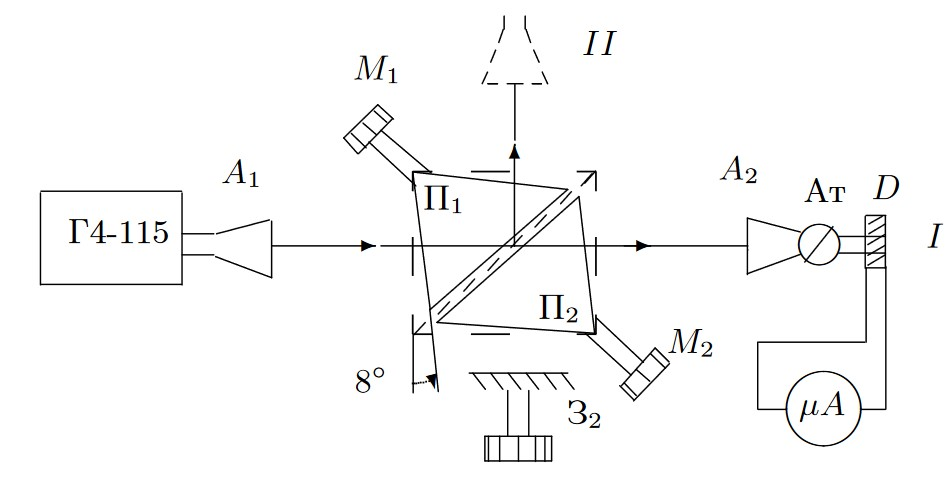
\includegraphics[scale=0.5]{../images/462_6}
\end{figure}

\section{Проведение эксперимента}

\begin{enumerate}

\setcounter{enumi}{0}

\item Настроим генератор, руководствуясь техническим описанием.

\item Установим столик с призмами так, чтобы воздушный зазор был ориентирован под углом $45^\circ$ к падающему лучу.
 
\item Расположим приемную антенну на одной прямой с передатчиком и снимем металлическое зеркало. Добьемся максимального отклика микроамперметра, поворачивая столик и приемную антенну. Закрепим столик.

\item Вращением ручек генератора настроимся на максимальную выходную мощность клистрона.

\item Добьемся загорания сигнальной лампочки и определим рабочаю частоту клистрона -- $37.08\ ГГц$. Соответствующая длина волны -- $8.1\ мм$.

\end{enumerate}

\section{Обработка данных}

\begin{enumerate}

\setcounter{enumi}{5}

\item Снимем зависимость интенсивности прошедшей длины волны от величины зазора. Построим график зависимости интенсивности от величины зазора.

\begin{figure}[H]
\centering
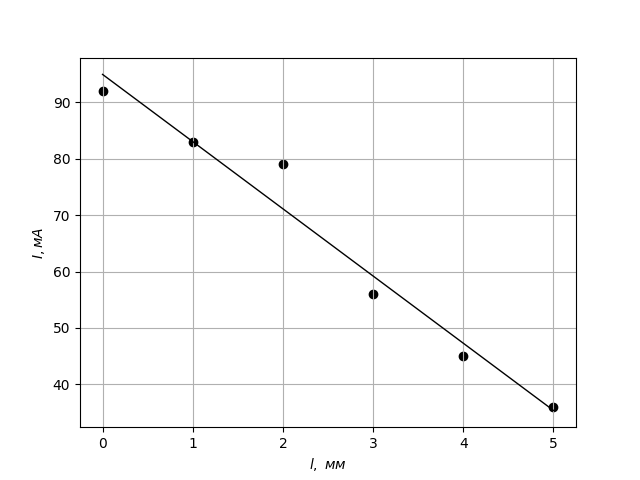
\includegraphics[scale=0.5]{../images/462_1.png}
\end{figure}

\item Переставим приемник для измерения отраженного сигнала. Снимем зависимость интенсивности отраженной волны от величины зазора.

\begin{figure}[H]
\centering
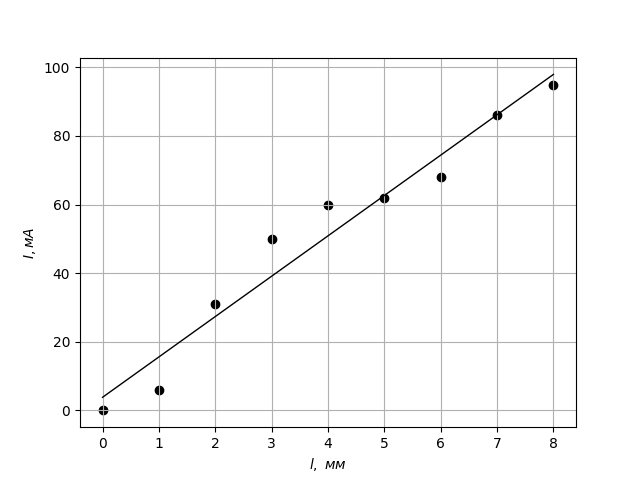
\includegraphics[scale=0.5]{../images/462_2.png}
\end{figure}

\item Установим такую величину зазора, при которой ток равен половине максимального

\item Построим графики зависимости коэффициентов $T$ и $R$ от величины зазора $l$, отнормировав токи на максимальную величину.

\begin{figure}[H]
\centering
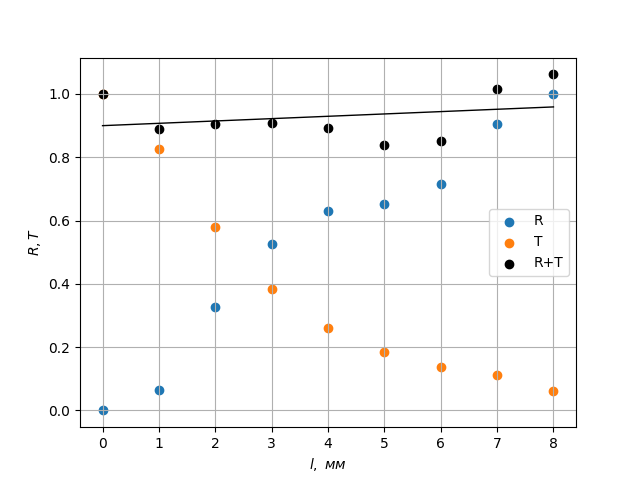
\includegraphics[scale=0.5]{../images/462_3.png}
\end{figure}

Примерно выполняется соотношение $R+T=1$.

\item Построим график $\ln{T}=f(z)$, где $z$ -- показания микрометра.

\begin{figure}[H]
\centering
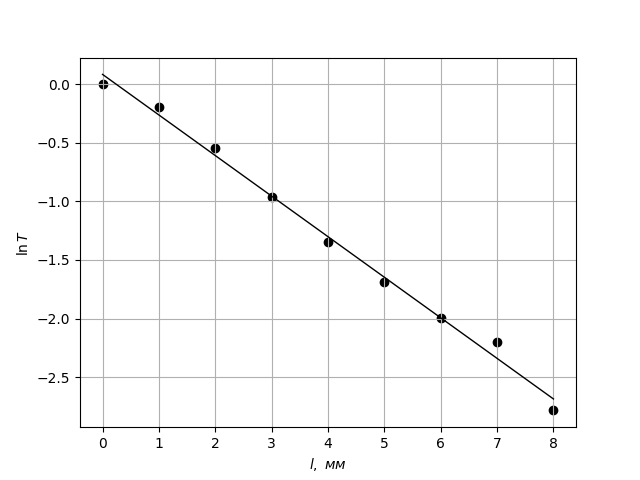
\includegraphics[scale=0.5]{../images/462_4.png}
\end{figure}

По наклону прямой, проведенной через полученные точки рассчитаем длину затухания $\Delta$:
\[\Delta=-1/k=2.9\ мм\]
Также величину $n\sin{\phi_1}$:
\[n\sin{\phi_1}=1+\left(\frac{\lambda}{4\pi\Lambda}\right)^2=1.05\]

Рассчитаем величину показателя преломления фторопласта $n$ учитывая, что $\phi_1\approx\frac{\pi}{4}$: $n=1.48$.

\item Соберем схему интерферометра Майкельсона, используя в качестве разделителя воздушный зазор между фильтрами.

\item Снимем зависимость тока от координаты подвижного зеркала. Определим экспериментальное значение длины волны. 

\begin{figure}[H]
\centering
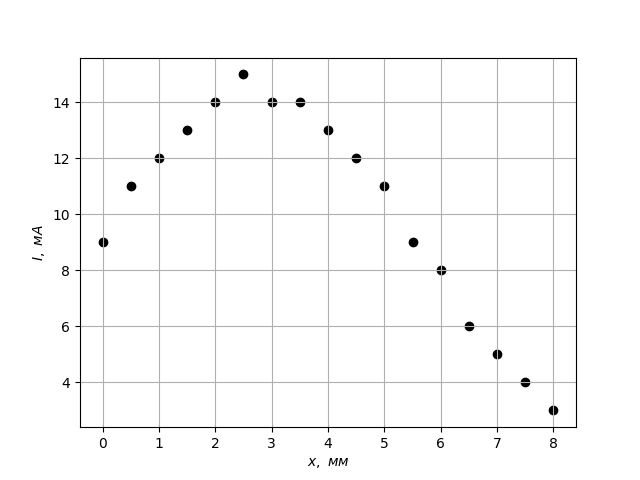
\includegraphics[scale=0.5]{../images/462_5.png}
\end{figure}

Показания повторяются при $x=5.5\ мм$. Следовательно, $\lambda=2x=11\ мм$.

\item Для измерения показателя преломления фторопласта настроим интерферометр на максимальную интенсивность и поместим пластину известной толщины перед неподвижным зеркалом. Подвижным зеркалом скомпенсируем возникшую длину оптического пути ($\delta x\approx4\ мм$).
\[n=1+\frac{\delta x}{h}\approx1.64\]
где $h=6.2\ мм$ -- толщина пластины.

\end{enumerate}

\section{Вывод}

Значения показателя преломления фторопласта, полученные методом туннелирования и интерференционным методом отличаются, причем метод туннелирования привел нас значительно ближе к действительному значению показателя преломления.

\end{document}